%!TEX program = xelatex
\documentclass[11pt]{beamer}

\usepackage{amsfonts}
\usepackage{amsmath}
\usepackage{blindtext}
\usepackage{enumitem}
\usepackage{fancyvrb}

\usetheme{SaoPaulo}

\title{Python Basics!}
\subtitle{mutability, container methods}
\author{CS101 Lecture \#9}
\date{2016-10-26}

\setcounter{showSlideNumbers}{1}

\begin{document}
  \setcounter{showProgressBar}{0}
  \setcounter{showSlideNumbers}{0}

%%%%%%%%%%%%%%%%%%%%%%%%%%%%%%%%%%%%%%%%%%%%%%%%%%%%%%%%%%%%%%%%%%%%%%%%%%%%%%%%
\frame{\titlepage}

%%%%%%%%%%%%%%%%%%%%%%%%%%%%%%%%%%%%%%%%%%%%%%%%%%%%%%%%%%%%%%%%%%%%%%%%%%%%%%%%
\setcounter{framenumber}{0}
\setcounter{showProgressBar}{1}
\setcounter{showSlideNumbers}{1}


%%%%%%%%%%%%%%%%%%%%%%%%%%%%%%%%%%%%%%%%%%%%%%%%%%%%%%%%%%%%%%%%%%%%%%%%%%%%%%%%
\section{\texttt{for} loops}

%%%%%%%%%%%%%%%%%%%%%%%%%%%%%%%%%%%%%%%%%%%%%%%%%%%%%%%%%%%%%%%%%%%%%%%%%%%%%%%%
\begin{frame}[fragile]
  \frametitle{Example}
  \Enlarge

  \begin{semiverbatim}
for i in range(10):
    print(i ** 2) \pause

for i in range(2,10):
    print(i ** 2) \pause

for i in range(2,10,3):
    print(i ** 2)

  \end{semiverbatim}
\end{frame}

%%%%%%%%%%%%%%%%%%%%%%%%%%%%%%%%%%%%%%%%%%%%%%%%%%%%%%%%%%%%%%%%%%%%%%%%%%%%%%%%
\section{Mutability \& Aliasing}

%%%%%%%%%%%%%%%%%%%%%%%%%%%%%%%%%%%%%%%%%%%%%%%%%%%%%%%%%%%%%%%%%%%%%%%%%%%%%%%%
\begin{frame}[fragile]
  \frametitle{Example}
  \Enlarge

  \begin{semiverbatim}
x = 1
y = x
y = 2
# what is x? %\pause

x = [ 1,2,3 ]
y = x
y[0] = 6
# what is x?
  \end{semiverbatim}
\end{frame}

%%%%%%%%%%%%%%%%%%%%%%%%%%%%%%%%%%%%%%%%%%%%%%%%%%%%%%%%%%%%%%%%%%%%%%%%%%%%%%%%
\begin{frame}[fragile]
  \frametitle{Mutability}
  \Enlarge

  \begin{itemize}
  \myitem  We distinguished \emph{mutability} and \emph{immutability}. %\pause
  \myitem  The distinction arises from the storage in memory.
  \end{itemize}
\end{frame}

%%%%%%%%%%%%%%%%%%%%%%%%%%%%%%%%%%%%%%%%%%%%%%%%%%%%%%%%%%%%%%%%%%%%%%%%%%%%%%%%
\begin{frame}[fragile]
  \frametitle{Mutability}
  \Enlarge

  \begin{itemize}
  \myitem  \emph{Immutability} occurs when values are copies in memory.
  \end{itemize}
  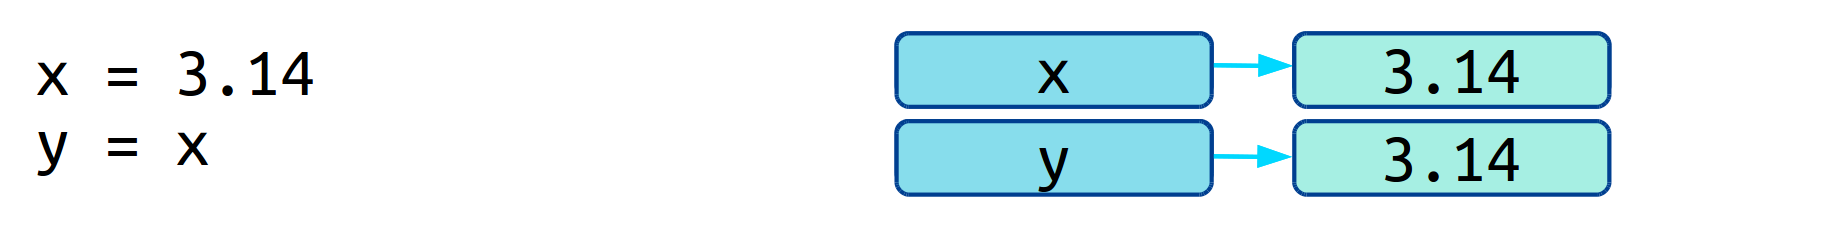
\includegraphics[width=0.8\textwidth]{./img/memory-immutability.png} \\
  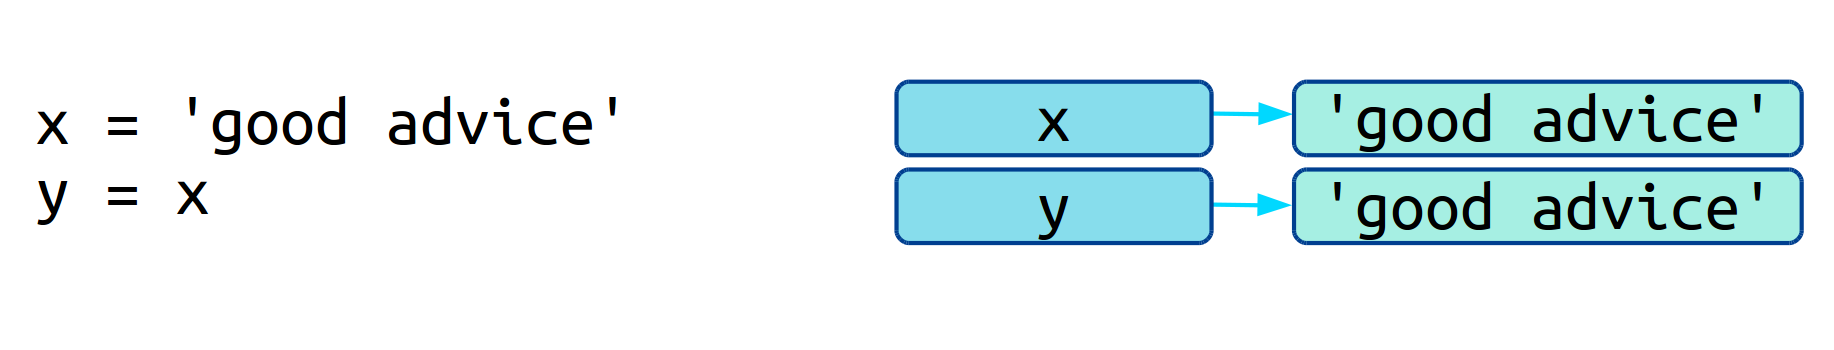
\includegraphics[width=0.8\textwidth]{./img/memory-immutability-string.png}
\end{frame}

%%%%%%%%%%%%%%%%%%%%%%%%%%%%%%%%%%%%%%%%%%%%%%%%%%%%%%%%%%%%%%%%%%%%%%%%%%%%%%%%
\begin{frame}[fragile]
  \frametitle{Mutability \& immutability}
  \Enlarge

  \begin{itemize}
  \myitem  \emph{Mutability} occurs when values share the same location. %\pause
  \myitem  The distinction arises from the storage in memory.
  \end{itemize}
  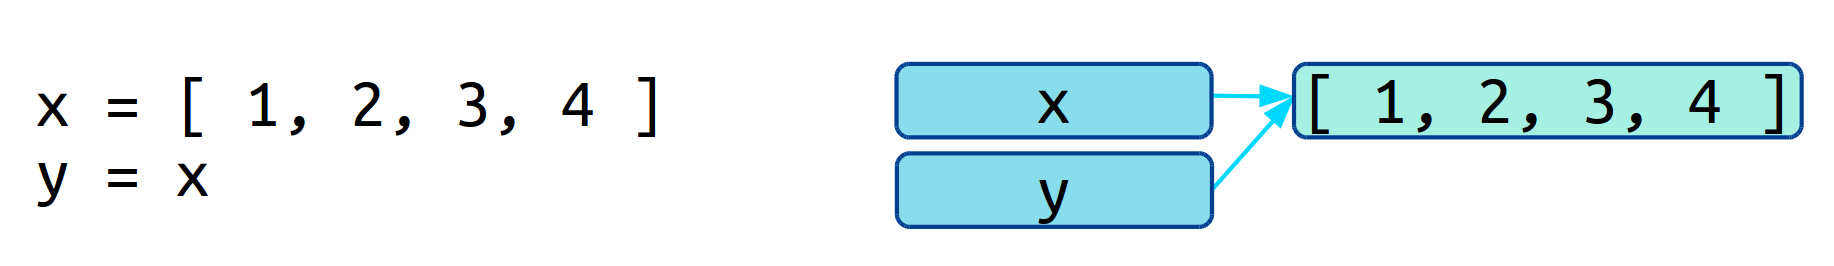
\includegraphics[width=0.8\textwidth]{./img/memory-mutability.png}
\end{frame}

%%%%%%%%%%%%%%%%%%%%%%%%%%%%%%%%%%%%%%%%%%%%%%%%%%%%%%%%%%%%%%%%%%%%%%%%%%%%%%%%
\begin{frame}[fragile]
  \frametitle{Aliasing}
  \Enlarge

  \begin{itemize}
  \myitem  \emph{Aliasing} occurs when one memory location has two names. %\pause
  \myitem  \textcolor{red}{Aliasing causes mutable types to behave unexpectedly!}
  \end{itemize}
  \begin{semiverbatim}

  \end{semiverbatim}
\end{frame}

%%%%%%%%%%%%%%%%%%%%%%%%%%%%%%%%%%%%%%%%%%%%%%%%%%%%%%%%%%%%%%%%%%%%%%%%%%%%%%%%
\begin{frame}[fragile]
  \frametitle{Aliasing}
  \Enlarge

  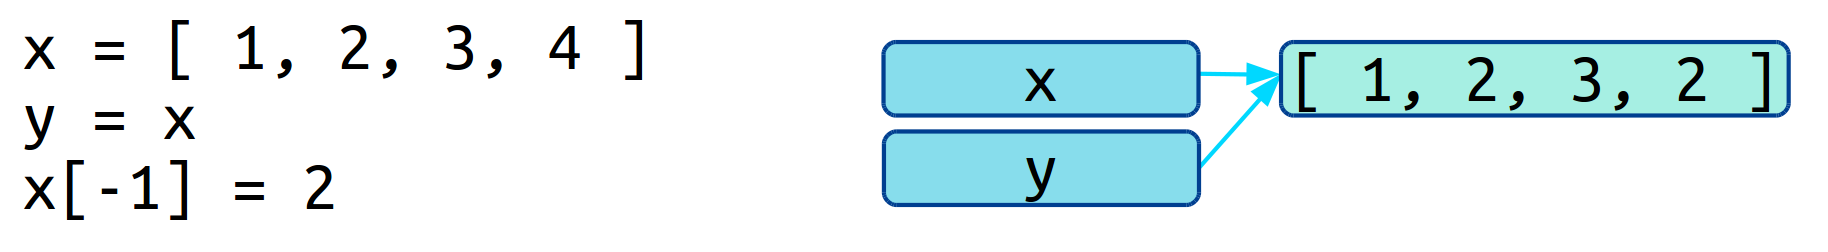
\includegraphics[width=0.8\textwidth]{./img/memory-aliasing.png}
\end{frame}

%%%%%%%%%%%%%%%%%%%%%%%%%%%%%%%%%%%%%%%%%%%%%%%%%%%%%%%%%%%%%%%%%%%%%%%%%%%%%%%%
\begin{frame}[fragile]
  \frametitle{Example}
  \Enlarge

  \begin{semiverbatim}
x = [ 1,2,3 ]
y = x
y[0] = 6
# what is x?
  \end{semiverbatim}
\end{frame}

%%%%%%%%%%%%%%%%%%%%%%%%%%%%%%%%%%%%%%%%%%%%%%%%%%%%%%%%%%%%%%%%%%%%%%%%%%%%%%%%
\begin{frame}[fragile]
  \frametitle{Example}
  \Enlarge

  \begin{semiverbatim}
a = [ 'a', 'b', 'c', 'd' ]
b = a
b[3] = '*'
  \end{semiverbatim}
  What is the final value of \texttt{a}?
  \begin{enumerate}[label=\Alph*]
  \item  \texttt{[ 'a', 'b', '*', 'd' ]}
  \item  \texttt{[ 'a', 'b', 'c', '*' ]}  %$\star$
  \item  \texttt{[ 'a', 'b', 'c', 'd' ]}
  \item  None of the above.
  \end{enumerate}
\end{frame}

%%%%%%%%%%%%%%%%%%%%%%%%%%%%%%%%%%%%%%%%%%%%%%%%%%%%%%%%%%%%%%%%%%%%%%%%%%%%%%%%
\begin{frame}[fragile]
  \frametitle{Tuples}
  \Enlarge

  \begin{itemize}
  \myitem  The immutable analogue of a \texttt{list} is a \texttt{tuple}. %\pause
  \myitem  We form a tuple by using parentheses \texttt{()} instead of square brackets \texttt{[]}.
  \end{itemize}
\end{frame}

%%%%%%%%%%%%%%%%%%%%%%%%%%%%%%%%%%%%%%%%%%%%%%%%%%%%%%%%%%%%%%%%%%%%%%%%%%%%%%%%
\begin{frame}[fragile]
  \frametitle{Where can I use tuples?}
  \Enlarge

  \begin{itemize}
  \myitem  \texttt{tuple}s can be used to format multiple values for \texttt{print}.
  \end{itemize}
  \begin{semiverbatim}
'%i %i %i' % (1,2,3)
  \end{semiverbatim}
\end{frame}

%%%%%%%%%%%%%%%%%%%%%%%%%%%%%%%%%%%%%%%%%%%%%%%%%%%%%%%%%%%%%%%%%%%%%%%%%%%%%%%%
\begin{frame}[fragile]
  \frametitle{Example}
  \Enlarge

  \begin{semiverbatim}
s = ???
x = 10
y = 'Hello'
z = 3.14
print(s % x,y,z)
  \end{semiverbatim}
  What should replace the \texttt{???}?
  \begin{enumerate}[label=\Alph*]
  \item  \texttt{'\%i \%f \%s'}
  \item  \texttt{'\%f \%s \%i'}
  \item  \texttt{'\%i \%s \%f'} % $\star$
  \item  None of the above.
  \end{enumerate}
\end{frame}

%%%%%%%%%%%%%%%%%%%%%%%%%%%%%%%%%%%%%%%%%%%%%%%%%%%%%%%%%%%%%%%%%%%%%%%%%%%%%%%%
\begin{frame}[fragile]
  \frametitle{Where can I use tuples?}
  \Enlarge

  \begin{itemize}
  \myitem  \texttt{tuple}s can also be used on the left-hand side of an assignment operator. %\pause
  \myitem  This lets us make \emph{multiple assignments} at once. %\pause
  \end{itemize}
  \begin{semiverbatim}
one,pi,hello = ( 1,3.14,'Hi' ) \pause
x,y = y,x
  \end{semiverbatim}
\end{frame}

%%%%%%%%%%%%%%%%%%%%%%%%%%%%%%%%%%%%%%%%%%%%%%%%%%%%%%%%%%%%%%%%%%%%%%%%%%%%%%%%
\begin{frame}[fragile]
  \frametitle{Where can I use tuples?}
  \Enlarge

  \begin{itemize}
  \myitem  \texttt{tuple}s can return \emph{multiple values} from a function. %\pause
  \end{itemize}
  \begin{semiverbatim}
def fun():
    return 'hi', 3, 'lo'

a,b,c = fun()
  \end{semiverbatim}
\end{frame}

%%%%%%%%%%%%%%%%%%%%%%%%%%%%%%%%%%%%%%%%%%%%%%%%%%%%%%%%%%%%%%%%%%%%%%%%%%%%%%%%
\section{Container Methods}

%%%%%%%%%%%%%%%%%%%%%%%%%%%%%%%%%%%%%%%%%%%%%%%%%%%%%%%%%%%%%%%%%%%%%%%%%%%%%%%%
\begin{frame}[fragile]
  \frametitle{Container Methods}
  \Enlarge

  \begin{itemize}
  \myitem  Because \texttt{list}s are mutable, we can change their contents. %\pause
  \end{itemize}
  \begin{semiverbatim}
x = [ 4,1,2,3 ]
x[3] = -2       # item assignment
x.append(5)     # appending items
del x[1]        # removing items
x.sort()        # changing item order
  \end{semiverbatim}
\end{frame}

%%%%%%%%%%%%%%%%%%%%%%%%%%%%%%%%%%%%%%%%%%%%%%%%%%%%%%%%%%%%%%%%%%%%%%%%%%%%%%%%
\begin{frame}[fragile]
  \frametitle{Container Methods}
  \Enlarge

  \begin{itemize}
  \myitem  \texttt{sort} and \texttt{append} modify the \texttt{list} itself. %\pause
  \end{itemize}
  \begin{alertblock}{Warning!}
  This explains why \texttt{sort} and \texttt{append} \texttt{return None}!
  \end{alertblock}
  \begin{semiverbatim}
x = [ 4,1,2,3 ]
x.sort()   # This is the right way to sort a list.
print(x)
  \end{semiverbatim}
\end{frame}

%%%%%%%%%%%%%%%%%%%%%%%%%%%%%%%%%%%%%%%%%%%%%%%%%%%%%%%%%%%%%%%%%%%%%%%%%%%%%%%%
\begin{frame}[fragile]
  \frametitle{Container Methods}
  \Enlarge

  \begin{itemize}
  \myitem  \texttt{sort}, \texttt{reverse}, and \texttt{append} modify the \texttt{list} itself.
  \end{itemize}
  \begin{alertblock}{Warning!}
  This explains why \texttt{sort} and \texttt{append} \texttt{return None}!
  \end{alertblock}
  \begin{semiverbatim}
x = [ 4,1,2,3 ]
x = x.sort() # MANY of you will do this wrong way!
print(x)
  \end{semiverbatim}
\end{frame}

%%%%%%%%%%%%%%%%%%%%%%%%%%%%%%%%%%%%%%%%%%%%%%%%%%%%%%%%%%%%%%%%%%%%%%%%%%%%%%%%
\begin{frame}[fragile]
  \frametitle{Example}
  \Enlarge

  \begin{semiverbatim}
y = [ 3,2,1 ]
x = y.append( 5 )
y[-1] = 3
  \end{semiverbatim}
  What is the final value of \texttt{x}?
  \begin{enumerate}[label=\Alph*]
  \item  \texttt{[ 3, 2, 1, 3 ]}
  \item  \texttt{[ 3, 2, 1, 5 ]}
  \item  \texttt{[ 3, 2, 1 ]}
  \item  \texttt{None}
  \end{enumerate}
\end{frame}

%%%%%%%%%%%%%%%%%%%%%%%%%%%%%%%%%%%%%%%%%%%%%%%%%%%%%%%%%%%%%%%%%%%%%%%%%%%%%%%%
\begin{frame}[fragile]
  \frametitle{Container Methods}
  \Enlarge

  \begin{itemize}
  \myitem  \texttt{index} returns the index of the first occurrence of a value in a \texttt{list}.
  \myitem  \texttt{count} returns how many times a value occurs.
  \myitem  \texttt{in} returns membership in the \texttt{list}.
  \myitem  \texttt{*} \emph{repeats} a \texttt{list}.
  \myitem  \texttt{+} \emph{extends} a \texttt{list} (also \texttt{extend})..
  \myitem  \texttt{max}, \texttt{min}, \texttt{len}, etc.
  \end{itemize}
\end{frame}

%%%%%%%%%%%%%%%%%%%%%%%%%%%%%%%%%%%%%%%%%%%%%%%%%%%%%%%%%%%%%%%%%%%%%%%%%%%%%%%%
\section{String/List Methods}

%%%%%%%%%%%%%%%%%%%%%%%%%%%%%%%%%%%%%%%%%%%%%%%%%%%%%%%%%%%%%%%%%%%%%%%%%%%%%%%%
\begin{frame}[fragile]
  \frametitle{\texttt{string.split} method}
  \Enlarge

  \begin{itemize}
  \myitem  \texttt{split} returns a \texttt{list}. %\pause
  \myitem  Takes a single string argument, the \emph{delimiter}. %\pause
  \end{itemize}
  \begin{semiverbatim}
name = 'Oliver Wendell Holmes'
names = name.split(' ')
print(names[-1])
  \end{semiverbatim}
\end{frame}

%%%%%%%%%%%%%%%%%%%%%%%%%%%%%%%%%%%%%%%%%%%%%%%%%%%%%%%%%%%%%%%%%%%%%%%%%%%%%%%%
\begin{frame}[fragile]
  \frametitle{Example}
  \Enlarge

  \begin{semiverbatim}
x = 'A+B+C'
y = x.split()
  \end{semiverbatim}
  What is the final value of \texttt{y}?
  \begin{enumerate}[label=\Alph*]
  \item  \texttt{'ABC'}
  \item  \texttt{[ 'A','B','C' ]}
  \item  \texttt{[ 'A+B+C' ]} % $\star$
  \item  \texttt{'A','B','C'}
  \item  \texttt{None}
  \end{enumerate}
\end{frame}

%%%%%%%%%%%%%%%%%%%%%%%%%%%%%%%%%%%%%%%%%%%%%%%%%%%%%%%%%%%%%%%%%%%%%%%%%%%%%%%%
\begin{frame}[fragile]
  \frametitle{Example}
  \Enlarge

  \begin{semiverbatim}
x = 'A+B+C'
y = x.split('+')
  \end{semiverbatim}
  What is the final value of \texttt{y}?
  \begin{enumerate}[label=\Alph*]
  \item  \texttt{'ABC'}
  \item  \texttt{[ 'A','B','C' ]} % $\star$
  \item  \texttt{[ 'A+B+C' ]}
  \item  \texttt{'A','B','C'}
  \item  \texttt{None}
  \end{enumerate}
\end{frame}

%%%%%%%%%%%%%%%%%%%%%%%%%%%%%%%%%%%%%%%%%%%%%%%%%%%%%%%%%%%%%%%%%%%%%%%%%%%%%%%%
\begin{frame}[fragile]
  \frametitle{Example}
  \Enlarge

  \begin{semiverbatim}
x = 'A+B+C'
y = x.split('-')
  \end{semiverbatim}
  What is the final value of \texttt{y}?
  \begin{enumerate}[label=\Alph*]
  \item  \texttt{'A+B+C'}
  \item  \texttt{[ 'A+B+C' ]} % $\star$
  \item  \texttt{( 'A+B+C' )}
  \item  \texttt{None}
  \end{enumerate}
\end{frame}

%%%%%%%%%%%%%%%%%%%%%%%%%%%%%%%%%%%%%%%%%%%%%%%%%%%%%%%%%%%%%%%%%%%%%%%%%%%%%%%%
\begin{frame}[fragile]
  \frametitle{Example}
  \Enlarge

  \begin{semiverbatim}
x = '+A+B+C+'
y = x.split('+')
  \end{semiverbatim}
  What is the final value of \texttt{y}?
  \begin{enumerate}[label=\Alph*]
  \item  \texttt{'ABC'}
  \item  \texttt{[ 'A','B','C' ]}
  \item  \texttt{[ '','A','B','C','' ]} % $\star$
  \item  \texttt{[ 'A+B+C' ]}
  \item  \texttt{None}
  \end{enumerate}
\end{frame}

%%%%%%%%%%%%%%%%%%%%%%%%%%%%%%%%%%%%%%%%%%%%%%%%%%%%%%%%%%%%%%%%%%%%%%%%%%%%%%%%
\begin{frame}[fragile]
  \frametitle{\texttt{string.join} method}
  \Enlarge

  \begin{itemize}
  \myitem  \texttt{join} returns a \texttt{str}. %\pause
  \myitem  Takes a single \texttt{list} argument. %\pause
  \myitem  Returns the \texttt{list} elements joined as a string. %\pause
  \end{itemize}
  \begin{semiverbatim}
names = [ "Geoffrey", "Richard",
          "Aloysius", "Johnston" ]
#  GOAL:  """Geoffrey Richard
#            Aloysius Johnston""" %\pause
' '.join(names)     # note the odd syntax!
                    # join is a STRING method
  \end{semiverbatim}
\end{frame}

%%%%%%%%%%%%%%%%%%%%%%%%%%%%%%%%%%%%%%%%%%%%%%%%%%%%%%%%%%%%%%%%%%%%%%%%%%%%%%%%
\begin{frame}[fragile]
  \frametitle{Example}
  \Enlarge

  \begin{semiverbatim}
a = [ 'X', 'A', 'G' ]
b = a[:]
a.sort()
x = ','.join(b)
  \end{semiverbatim}
  What is the final value of \texttt{x}?
  \begin{enumerate}[label=\Alph*]
  \item  \texttt{'XAG'}
  \item  \texttt{[ 'X,A,G' ]}
  \item  \texttt{'A,G,X'}
  \item  \texttt{',A,G,X,'}
  \item  \texttt{'X,A,G'} % $\star$
  \end{enumerate}
\end{frame}

%%%%%%%%%%%%%%%%%%%%%%%%%%%%%%%%%%%%%%%%%%%%%%%%%%%%%%%%%%%%%%%%%%%%%%%%%%%%%%%%
\begin{frame}[fragile]
  \frametitle{One more thing...}
  \Enlarge

  \begin{Verbatim}
range( 0, 6, 2 )
list( range( 0, 6, 2 ) ) 

out: [ 0, 2, 4 ]
  \end{Verbatim}
\end{frame}

%%%%%%%%%%%%%%%%%%%%%%%%%%%%%%%%%%%%%%%%%%%%%%%%%%%%%%%%%%%%%%%%%%%%%%%%%%%%%%%%
\section{Reminders}

%%%%%%%%%%%%%%%%%%%%%%%%%%%%%%%%%%%%%%%%%%%%%%%%%%%%%%%%%%%%%%%%%%%%%%%%%%%%%%%%
\begin{frame}
  \frametitle{Reminders}
  \Enlarge

 \begin{itemize}
 	\myitem  Homework \#3 is due Wed Oct. 26.
 	\myitem  Homework \#4 is due Wed Nov.\ 4.
 	\myitem Midterm \#1 will be on the day of the 12th lecture (Nov. 7 Monday), covering through Lecture \#11. (evening)
 \end{itemize}
\end{frame}

\end{document}
